\TOWRITE{ALL}{Proofread WP 1 Management pass 1}
\begin{draft}
\TOWRITE{PS (Work Package Lead)}{For WP leaders, please check the following (remove items
once completed)}
\begin{verbatim}
- [ ] have all the tasks in this Work Package a lead institution?
- [ ] have all deliverables in the WP a lead institution?
- [ ] do all tasks list all sites involved in them?
- [ ] does the table of sites and their PM efforts match lists of sites for each task?
      (each site from the table is listed in all relevant tasks, and no site is listed
      only in the table or only at some task)
\end{verbatim}
\end{draft}

\begin{workpackage}[id=applications,wphases=0-48,swsites,
  title=Science demonstrators,
  short=Demonstrators,
  lead=XFEL,
  EGIRM=7,
  CDSRM=12,
  INSERMRM=24,
  QSRM=6,
  SILRM=12,
  SRLRM=9,
  UIORM=12,
  UPSUDRM=20,
  WTTRM=3,
  XFELRM=36,
  EPRM=3,
]
\begin{wpobjectives}
  The objectives of this work package are
 \begin{compactitem}
   \item to guide the development of core tools by simultaneously
     developing and using applications in diverse fields with active
     scientists from these fields, and
   \item to demonstrate that the tools we develop are valuable to diverse
     fields of science, thus ensuring we develop e-infrastructure and
     services which can cater for a broad customer base of EOSC.
   \end{compactitem}
\end{wpobjectives}

\begin{wpdescription}

  Whilst the components issued from work packages  \WPref{core} and \WPref{ecosystem} will be
  made available as generic building blocks for EOSC services, this
  work package aims at building and deploying bespoke EOSC services
  targeting real-world cases.

  We have selected a number of applications in a variety of domains
  to demonstrate the broad impact of \TheProject, in particular in the
  areas of astronomy
  (\localtaskref{astro}), education
  (\localtaskref{teaching}), fluid dynamics
  (\localtaskref{application-gpu}), geosciences
  (\localtaskref{geoscience}), health
  (\localtaskref{opendose-analysis}), mathematics
  (\localtaskref{math}) and photon science and imaging
  (\localtaskref{reproducibility-xfel}).
  The context and vision for each of the demonstrators is described in
  section \ref{sec:science-demonstrators-in-concept} on page
  \pageref{sec:science-demonstrators-in-concept}.

  Working closely with the core developers of the Jupyter ecosystem will make it possible to
  go way beyond what is normally available "out-of-the-box" and to offer better solutions,
  thereby guiding further development of the core features.

  \medskip
  Our demonstrators will typically undergo two-stages: (i)
  development and testing of the services locally at the developing partner
  site. (ii) Making the service available through the European Open
  Science Cloud (EOSC).

  All demonstrators will deliver base-line services by making the
  relevant notebooks executable in the \emph{European Binder Service} instance that this
  project will deployed on EOSC. This will demonstrate
  the Jupyter service capabilities such as reproducibility, interactive
  widget use and visualisation, and show how these can
  enable new open science on EOSC.

  The particular workflows, data infrastructures and data policies for
  FAIR\footnote{Findable, Accessible, Interoperable and Reusable} sharing of data vary from one community and use-case to
  the other, or may not be fully defined yet. Therefore, this proposal
  does not enforce a specific way of handling data. Instead we
  will explore in the demonstrator tasks how existing data policies,
  infrastructure and workflows can be respected and integrated with
  authentication and authorisation, data management, and
  JupyterHub/Binder services on EOSC. EGI is a partner
  for all the tasks in this work package and will work with us to find the
  best integration solutions in the evolving EOSC
  infrastructure.

  In the EOSC-hub project EGI operates a Jupyter Hub service which is deployed 
  in a scalable mode on EGI IaaS Cloud. This Jupyter Hub is already integrated 
  with the EUDAT B2DROP and OneData data management services of EOSC, and will 
  be integrated, in the next 12 months, with the EUDAT B2SHARE service.
  The integrations enable users to move data between Jupyter notebooks and storage 
  sites of the EGI Federation (with Onedata), between Jupyter and storage sites 
  of the EUDAT federation (B2SHARE), and between Jupyter and their personal cloud 
  storage hosted in EUDAT (B2DROP). The WP4 use cases will evaluate these data management 
  integrations and EGI will bring the respective technology from EOSC-hub into the 
  services operated by \TheProject.

  For some of the demonstrators, authentication and authorization and/or
  data management are being addressed outside \TheProject.
  This is for instance the case for the photon science and astronomy
  demonstrators via \href{https://panosc-eu.github.io/}{PaNOSC} and
  \href{https://www.eso.org/public/announcements/ann18084/}{ESCAPE} projects, respectively.

\end{wpdescription}

\begin{tasklist}
% add tasks from task directory here
% \begin{sitedescription}{XXX}

% PIC:
% see: http://ec.europa.eu/research/participants/portal/desktop/en/organisations/
%
% See ../proposal.tex, section Members of the Consortium for a
% complete description of what should go there

\subsubsection*{Curriculum vitae}
\TODO{AK - rules say "CV or description of the profile of the persons"
  can we name it "Track record" instead of CV?}

% Curriculum of the personnel at this institution. This includes
% to-be-hired people for which there is a tentative candidate.

%\input{CVs/First.Last.tex}
%\input{CVs/First.Last.tex}
%\input{CVs/First.Last.tex}

% For other to-be-hired person, please include here something like:
% \begin{participant}[type=res,PM=3,salary=5900]{NN}
%  <a _short_ description of the qualifications of whom you want to hire>
% \end{participant}

\subsubsection*{Publications, products, achievements}

\begin{compactenum}
\item \TOWRITE{XXX}{...}
\end{compactenum}

\subsubsection*{Relevant projects or activities}

\begin{compactenum}
\item \TOWRITE{XXX}{...}
\end{compactenum}

\subsubsection*{Significant infrastructure}

\TOWRITE{XXX}{...}
\end{sitedescription}
%%% Local Variables:
%%% mode: latex
%%% TeX-master: "../proposal"
%%% End:

\begin{task}[
  title=Co-design and technical support,
  id=codesign-support,
  lead=SRL,
  PM=15,
  wphases={1-48},
  partners={XFEL,EGI,CDS,INSERM,QS,SIL,UIO,UPSUD,WTT,EP}
]

This task coordinates and supports the work of the other \WPref{applications}
tasks. It will help us exploit synergies and coordinate the
gathering and formulation of requirements and the
preparation of the deliverables. It will also support demonstrator efforts to
speed-up the development process and ease the deployment of innovative
services. Finally, it will drive the co-design cycle between
\WPref{applications} and all the technical work packages
(\WPref{core}, \WPref{ecosystem} and \WPref{eosc}).

\begin{compactitem}
\item Assess co-design efforts and distribute workload across the core
  developers
\item Regularly feedback information to \WPref{education} to adapt
  trainings and dissemination
\item Offer technical support to the demonstrators throughout all the
  steps until final deployment of the services
\item Liase with \taskref{eosc}{eosc} for authentication,
  authorisation, data management and further EOSC integration.
\end{compactitem}

\end{task}

\begin{task}[
  title=Demonstrator: Astronomy,
  id=astro,
  lead=CDS,
  PM=18,
  wphases={18-42},
  partners={EGI,INSERM,QS,SRL,WTT,XFEL}
]

<<<<<<< HEAD
\textbf{Context}

  The Strasbourg Astronomical Data Center (CDS) is scientific data
  center hosted by the Observatory of Strasbourg. The CDS plays a unique and
  essential role in astronomy by adding value to published and reference data.
  CDS runs astronomical services that
  provide data for the world-wide astronomy research community. Its three main
  services (SIMBAD, VizieR and Aladin) are heavily used with up to one million
  queries per day.  These services are accessed through web interfaces, mainly
  for human interaction, as well as through programmatic interfaces, including
  the standardized protocols defined by the International Virtual Observatory
    Alliance \cite{ivoa}.

\begin{figure}[ht!]\centering
  \includegraphics[width=0.6\textwidth]{python-astro-citations}
  \caption{Mentions of programming languages in refereed Astronomy papers, extracted from ADS. Python usage has increased dramatically in the recent years.}\label{fig:python-astro-citations}
\end{figure}

  Python and notebooks are rapidly increasing in importance for astronomy
  research. Indeed, Python for Astronomy software ecosystem has known a
  constant steady growth in the latest years, as shown in
  figure~\ref{fig:python-astro-citations}. As Python and notebooks integrate
  well together, the Jupyter notebook as an analysis tool is becoming a hot
  topic in the astronomical world: large surveys like the LSST (Large Synoptic
  Survey Telescope) have endorsed the usage of the Jupyter platform for their
    data access portal \cite{lsst2017scienceplatform}.\\


  We will develop a Jupyter-based framework to efficiently access, explore,
  visualize and analyze reference data that are available through CDS services
  as a real example of using open astronomy data.
  We will provide scientific users with a set of customizable Jupyter notebooks
  for visualization and analysis tasks, providing a new level of
  interoperability with python libraries and notebooks as is highly demanded
  by the astronomy research community.

  The focus is on the two following user stories:
    \begin{compactitem}
        \item analysis of catalogue data results, up to billions of rows.
              Tabular data is the typical output of SIMBAD and VizieR data.
        \item modular dashboard-like interface providing a top level
              interactive view of the available data for a given astronomical
              object and enabling loading and analysis of those data.
    \end{compactitem}


  \textbf{This task}

  This task will build on existing Python libraries to access CDS data
=======
  This task (see page \pageref{sec:concept-demonstrator-astronomy} for
  context) will build on existing Python libraries to access CDS data
  \TODO{Recall what the acronym CDS stands for?}
>>>>>>> f429aa823b2ccd0fd77ca58a7ef1a9626d9e87d3
  (\textit{astroquery.[cds/simbad/vizier/xmatch]}). For visualization, we will
  use proven tools like \textit{GLUE} and \textit{ipyvolume}, which are now
  built upon the Jupyter stack.
  We will also make significant improvement to existing Jupyter widgets
  (\textit{ipyaladin}, interactive sky atlas running in the notebook) and
  develop a new widget to offer a tree-like view of available
  datasets.\TODO{will this be specific to certain needs in astronomy or general purpose?}

  We will also develop Python libraries to allow integration and usage in
  notebook of existing CDS infrastructure services, namely CDSLogin (which
  provides authentication) and CDS MyData (remote storage space for tabular
  data).
  This will allow the user to interact with one's personal storage space from
  the notebook. It will also allow for advanced customisation of the interface
  to fit user needs.

  The work is organised with a two stage approach. Firstly, the generated
  notebooks will run locally on user machines (representing a milestone for
  this task). Following the Binder development in \WPref{eosc}, we will aim
  to run these notebooks on the European Binder Service. The aspiration is
  that this contributes to the development of innovative services for the EOSC.
  The deliverable of this task will be a demonstrator available to the
  scientific user community (\localdelivref{demonstrators}).

  By milestone 3, astronomical data services based on reference
<<<<<<< HEAD
  astronomy data from CDS are made available in Jupyter notebooks, and
  decision point on how to use developments of \WPref{eosc} for running these
  notebooks on the European Binder Service.

\begin{figure}[ht!]\centering
  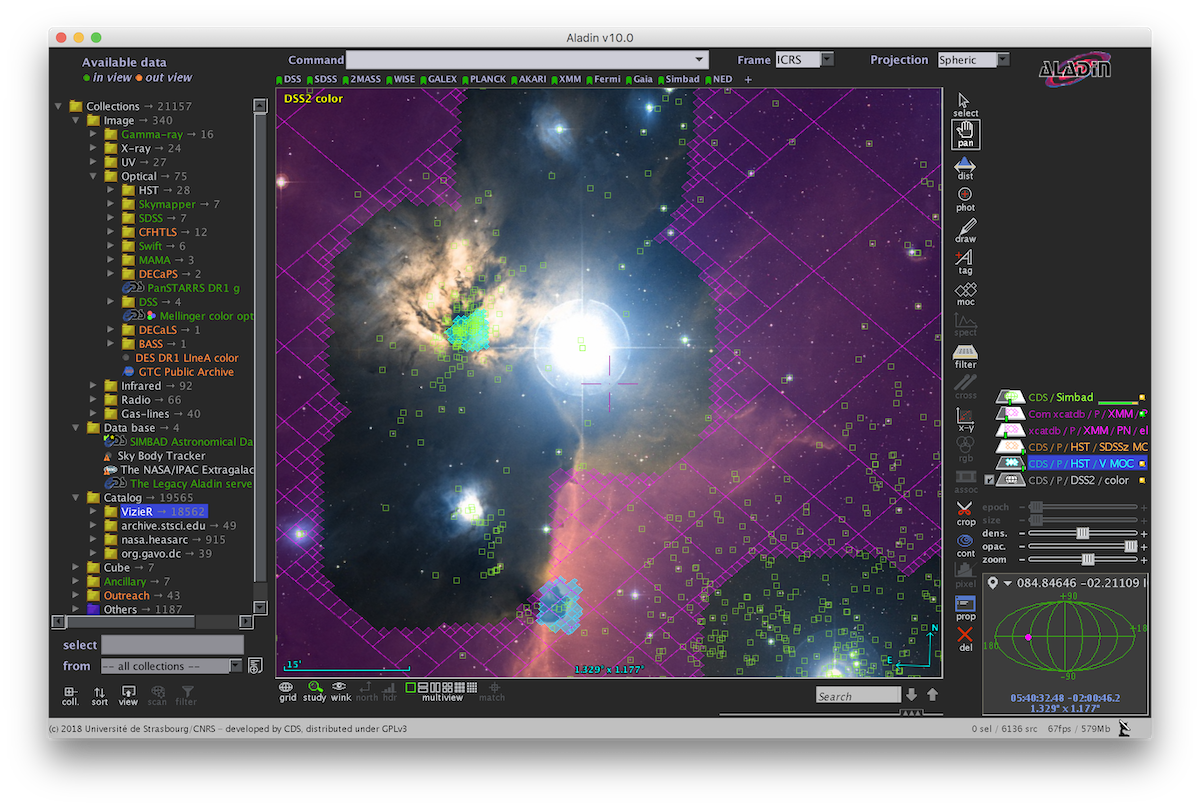
\includegraphics[width=1.0\textwidth]{astro-aladin-snapshot}
  \caption{Simbad objects, XMM and Hubble coverages overlaid on Digital Sky Survey imagery in the vicinity of the Horsehead nebula, and visualized in Aladin Desktop software.}\label{fig:astro-aladin-snapshot}
\end{figure}

  Access to the notebooks will be provided as a one-click action option from
  SIMBAD and VizieR results pages.
  Thus, providing with a one-click way of visualizing, filtering and analyzing
these potentially large tables will bridge the gap between access and analysis
of the data, with zero installation for the user.
  For specific science cases, we will explore rendering of notebooks with
  interactive widgets through "Voila", as to allow users not familiar with
  Python to benefit from the Jupyter notebook framework.
  Figure~\ref{fig:astro-aladin-snapshot} depicts typical data objects we want to analyse and interact with in the notebooks: images, catalogue data, datasets coverages.

  These new developments will be highly visible to the large number of astronomers who use the CDS services (50,000 unique visitors per month) and such tools are in high demand by these users.

  The CDS expertise in astronomy data and interfaces will be profitably combined with expertise of BOSSEE partners to ensure the deployment of high quality widgets (Simula, WildTree Tech, QuantStack).

  A demonstrator will be developed (Deliverable \localdelivref{application-astro}).

=======
  astronomy data from CDS will be made available in Jupyter notebooks, and
  decision point on how to use developments of WP5 for running these
  notebooks on \TheProject's EOSC services.
>>>>>>> f429aa823b2ccd0fd77ca58a7ef1a9626d9e87d3

  The work carried out in this task will be reported on in
  \delivref{applications}{applications-report}.
\end{task}

\begin{task}[
  title=Demonstrator: enriched teaching with Jupyter,
  id=teaching,
  lead=EP,
  PM=5, % EP: 3PM, UPSUD: 2PM, EuXFEL 1 PM
  wphases={0-48!.2},
  partners={EGI,INSERM,UIO,UPSUD,XFEL}
  ]


  In this task (see page \pageref{sec:concept-demonstrator-teaching}
  for context), we will \textbf{deliver and help deliver Jupyter-based
    courses at a large scale} in our own institutions, as a mean to
  \textbf{inform, evaluate, provide feedback on, and demonstrate the
    value of the work performed} in this project in the context of
  higher education, as well as to \textbf{develop and share best
    practices} and \textbf{demonstrate and disseminate} Jupyter's full
  potential for teaching.

  \'Ecole polytechnique and Université Paris-Sud are particularly well
  suited for this task because they
  \begin{enumerate}
  \item host a variety of local infrastructure (dedicated servers,
    local cloud, computer labs, ...);
  \item host a reactive community with highly qualified research
    software engineers (DevOps, software developers), researchers,
    professors, and students that have been working together on this
    topic for several years, with close collaboration between the two
    sites;
  \item offer very diverse courses, in many disciplines, and ranging
    from large lower undergraduate courses to specialized classes for
    graduate students and top notch engineers;
  \item have strong support from their respective teaching departments.
  \end{enumerate}

  The task will include the following activities
  \begin{compactitem}
  \item Reinforce the use of Jupyter technology in courses at
    all levels, notably in Mathematics and Data Science, in close
    collaboration between Ecole polytechnique and Université Paris Sud;
  \item Test the new developments and feed back to tasks
    \taskref{core}{jh-bh-conv}, \taskref{ecosystem}{xeus-cpp}, \taskref{ecosystem}{teaching-tools}, \taskref{applications}{math} and \taskref{eosc}{jh-bh-deployment};
  \item Follow up on a successful Jupyter day in
    2018~\footnote{\url{http://www.cmap.polytechnique.fr/~massot/Personal_web_page_of_Marc_Massot/JupyterX.html}}
    by organizing a yearly Jupyter event showcasing the latest
    advances for teaching and research;
  \item Foster sharing of experience, best practices and course
    material, at the local level, and then worldwide, through meetups,
    blogs, etc.
  \item Publish selected teaching material for interactive use on
    \TheProject's EOSC services (\delivref{applications}{demonstrators}).
  \end{compactitem}
  The work carried out will be reported on in
  \delivref{applications}{applications-report}.
\end{task}

\begin{task}[
  title=Application: Visualisation and control of fluid dynamics in Jupyter notebook,
  id=application-gpu,
  lead=SIL,
  PM=13,
  wphases={4-36},
  % don't include lead here
  partners={EGI}
]

\textbf{Context}

In recent years, the lattice Boltzmann method (LBM) emerged as an
interesting alternative to more established methods for fluid flow
simulations. Sailfish-cfd \cite{januszewski2014sailfish} is an open
source implementation of the LBM on General Purpose Graphical Processing
Unit (GPGPU) devices. It is written in Python with real-time
generation of CUDA-C code.  In order to harvest capabilities of GPGPUs
one needs to access the specialized hardware, which usually is
available to researchers as remote HPC resources.  The typical fluid
dynamics research workflow consists of three stages: preparing
boundary conditions, running a simulation, and data analysis. The
first and last stage require capable and responsive user interface for
maniputation and inspection of 3d data.  The Jupyter 3d visualisation
widgets developed in \taskref{ecosystem}{jupyter-widgets} can fulfil
such needs.

Based on previous experience with K3D-jupyter\cite{K3D}
widgets we know that web browser based software can display moderate
dataset during the simulation. As the dataset is becoming larger the
visualisation in the browser turns out to be nontrivial due to
limitations of the browser itself and required large data transfers. It is
an open question how much of data processing should be performed on
server-side and what can be done on the client hardware (i.e. in the
widget in the browser side of the user). Our
experience suggests that there is no clear answer and it depends on
the size of the data and its nature. For example, volume rendering
technique can be very effective on the browser side but infers large data
transfers. One can perform it the server-side, in a distributed way if
the simulation uses many nodes, but the interactivity is limited by
network latency. We will attempt to provide practical
solutions to this issue.
%


\textbf{This task}


In this task, we will contruct tools for editing and inspecting
boundary conditions. Having such tools as Jupyter widgets will allow
to complete the workflow without leaving Jupyter notebook. We plan the
following activities
\begin{compactitem}
\item Development of Jupyter notebooks using fluid
  simulation based on the high-performance Sailfish-cfd solver.
\item Implementing advanced widgets for data visualisation of large
  fluid dynamics simulations.
\item Implementing widgets for inspection and editing boundary
  conditions in LBM.
\end{compactitem}

This work will closely interact in with the task
\taskref{ecosystem}{jupyter-widgets}: it will both provide guidelines
for the development to \taskref{ecosystem}{jupyter-widgets} and serve
as test case for implemented features in
\taskref{ecosystem}{jupyter-widgets}.

The deliverable of this part will be a demonstrator
(\localdelivref{lbm-jupyter}) available via the EOSC hub, and
contributions to report \localdelivref{applications-report}.

\end{task}

\begin{task}[
  title=Demonstrator: Geosciences,
  id=geoscience,
  lead=UIO,
  PM=22,
  wphases={0-48},
  partners={EGI,QS,SRL,UPSUD}
]

% UPSud involvement: UPSud has a geoscience group (GEOPS) and will be
% interested in using the tools developed here. No formal PM.

The aim of this task (see page \pageref{sec:concept-demonstrators-geo}) is to build on the Jupyter ecosystem to create a standardized and shareable computing, data analysis and visualization framework for Geosciences. This task will focus on filling gaps that hinder open science and will include the following activities:

\emph{Visualization}

\begin{compactitem}
  \item Improvement upon existing mapping tools for specialized
    visualization of in-situ and model-generated data arizing in
    specific use cases (Land, river-runoff, ocean, ice, wave and
    atmosphere models, particle dispersion models, oil spill models,
    etc.).

  \item Improvements of the tooling for 3-D visualization of
    geographical datasets in the Jupyter notebook, for use cases such as
    displaying clouds, volcanic plumes, atmospheric rivers.
\end{compactitem}

\emph{Collaboration with Jupyter with specialized tools for earth sciences}

\begin{compactitem}
  \item adding the ability to interactively integrate information or corrections
    observed during field trips, correspdonding to specific geographical locations.

  \TODO{Concurrent editing links to real-time editing from the
    core WP2 - mention link?}

  \item adding the ability to deploy Jupyter-based applications together with
    the correspdonding execution environment, both in the form of a runnable
    notebook with \emph{Binder} or as a read-only yet interactive \emph{Voila}
    dashboard.
\end{compactitem}

This work will be carried out in two stages with first local development and deployment of \TheProject EOSC services for Geosciences 
(such as a BinderHub for Big data geosciences and \emph{voila} innovative interactive \emph{App}) and then deployment of these services on EOSC (\localdelivref{demonstrators}).
\end{task}

\begin{task}[
  title=Nuclear Medicine application,
  id=opendose-analysis,
  lead=INSERM,
  PM=25,
  wphases={3-33},
  partners={EGI,XFEL}
]

  \textbf{Context}

  % Scientific description
  Nuclear Medicine is a field of medicine where radioactive material
  (radiopharmaceutical) is used for diagnostic and therapy. Even though the
  majority of Nuclear Medicine procedures (90\% according to successive EANM
  surveys) are diagnostic examinations, therapeutic applications tend to
  develop and drag more and more attention, for example for the treatment of
  neuroendocrine tumours \cite{Bodei2009}.

  The formalism used to objectively characterise the irradiation process is
  similar for both application types: it was introduced in the late 60s by the
  MIRD (Medical Internal Radiation Dose) committee of the American Society of
  Nuclear Medicine (SNM). This formalism \cite{loevinger1991mird} requires two
  independent quantities; the radioisotope cumulated activity ($Bq.s$) in the
  source (tissue/organ) and the mean absorbed dose to a given target
  (tissue/organ) per radioisotope disintegration (S-value,
  $Gy.Bq^{-1}.s^{-1}$). The S-value calculation requires a clear definition of
  the geometry of the patient (or the model) and radioisotope decay
  characteristics, it can be expressed as a linear combination of
  yields/energies ($J$) and Specific Absorbed Fractions (SAF, $g^{-1}$).

  The calculation of SAFs involves radiation transport modelling and energy
  deposition scoring in anthropomorphic models, usually based on Monte Carlo
  simulation. Historically, SAFs were computed from mathematical models -
  simplistic approximations to human geometry. The advent of voxel-based
  computational models requires a new appraisal of dosimetric data. For
  example, the models recently proposed by the International Commission on
  Radiation Protection (ICRP) include 140 possible radiation sources, leading
  to around 20000 source/target combinations \cite{ICRP2009ICRPPhantoms}. The
  production of SAFs for these models for all possible source regions,
  radiation types and energiesimpul represent an important computation time
  (millions of CPU hours).

  The OpenDose project \cite{Chauvin2017} is a collaborative effort to generate
  reference dosimetric data using various Monte Carlo codes across different
  teams. The collaboration includes at the moment 14 research teams over 18
  institutes.  The idea is to trigger the collaborative development of a
  reference database, freely available, proposing dosimetric data applicable in
  a context of nuclear medicine dosimetry (for therapy and diagnostic
  applications). A major aspect of the project is the development of tools
  ensuring traceability and reproducibility of generated results.

  % Technical description
  OpenDose data is produced using the five most represented Monte Carlo
  simulation software in medical applications: Geant4/GATE, MCNP, EGS, PENELOPE
  and Fluka. Each simulation consists of calculating radiation transport in
  anthropomorphic models for specific parameters (source organ, particle type,
  energy, model and number of primaries to simulate). Every simulation produces
  binary (3D matrices) and ASCII files for a total of $\sim$150MB / simulation.
  The 3D matrices contain energy deposited per voxels, and ASCII files contain
  pre-processed data corresponding to energy deposited per regions such as
  organs and tissues. These raw outputs are later processed into dosimetric
  data such as Specific Absorbed Fractions (SAFs) and S-values.

  Producing data for one model (ex. adult female) requires $\sim$30,000
  simulations, with the workload shared between the different teams and
  software.

  The data produced by all the teams is currently centralised at the Cancer
  Research Center of Toulouse (CRCT), processed and fed into a local SQL
  database at CRCT.

  This collaborative effort raises some challenges:
  \begin{compactitem}
  \item Data production: a total of 750,000 hours of CPU time is needed per
    model.
  \item Volume of data: one model represents TB of raw data that can be
    heterogeneous from the different teams.
  \item Data analysis: raw data has to be processed into dosimetric data in a
    robust and reproducible way.
  \item Database: has to be efficient and handle all the data (raw and
    processed).
  \item Visualization: display and compare results from all teams.
  \end{compactitem}

  \textbf{This task}

  The objective of this task is to build on the Jupyter ecosystem to create a
  unified data analysis framework for the OpenDose project. Figure
  \ref{fig:opendose_framework} shows the overall framework of the project and
  how data will be managed.

  \begin{figure}[t!]
    \centering
    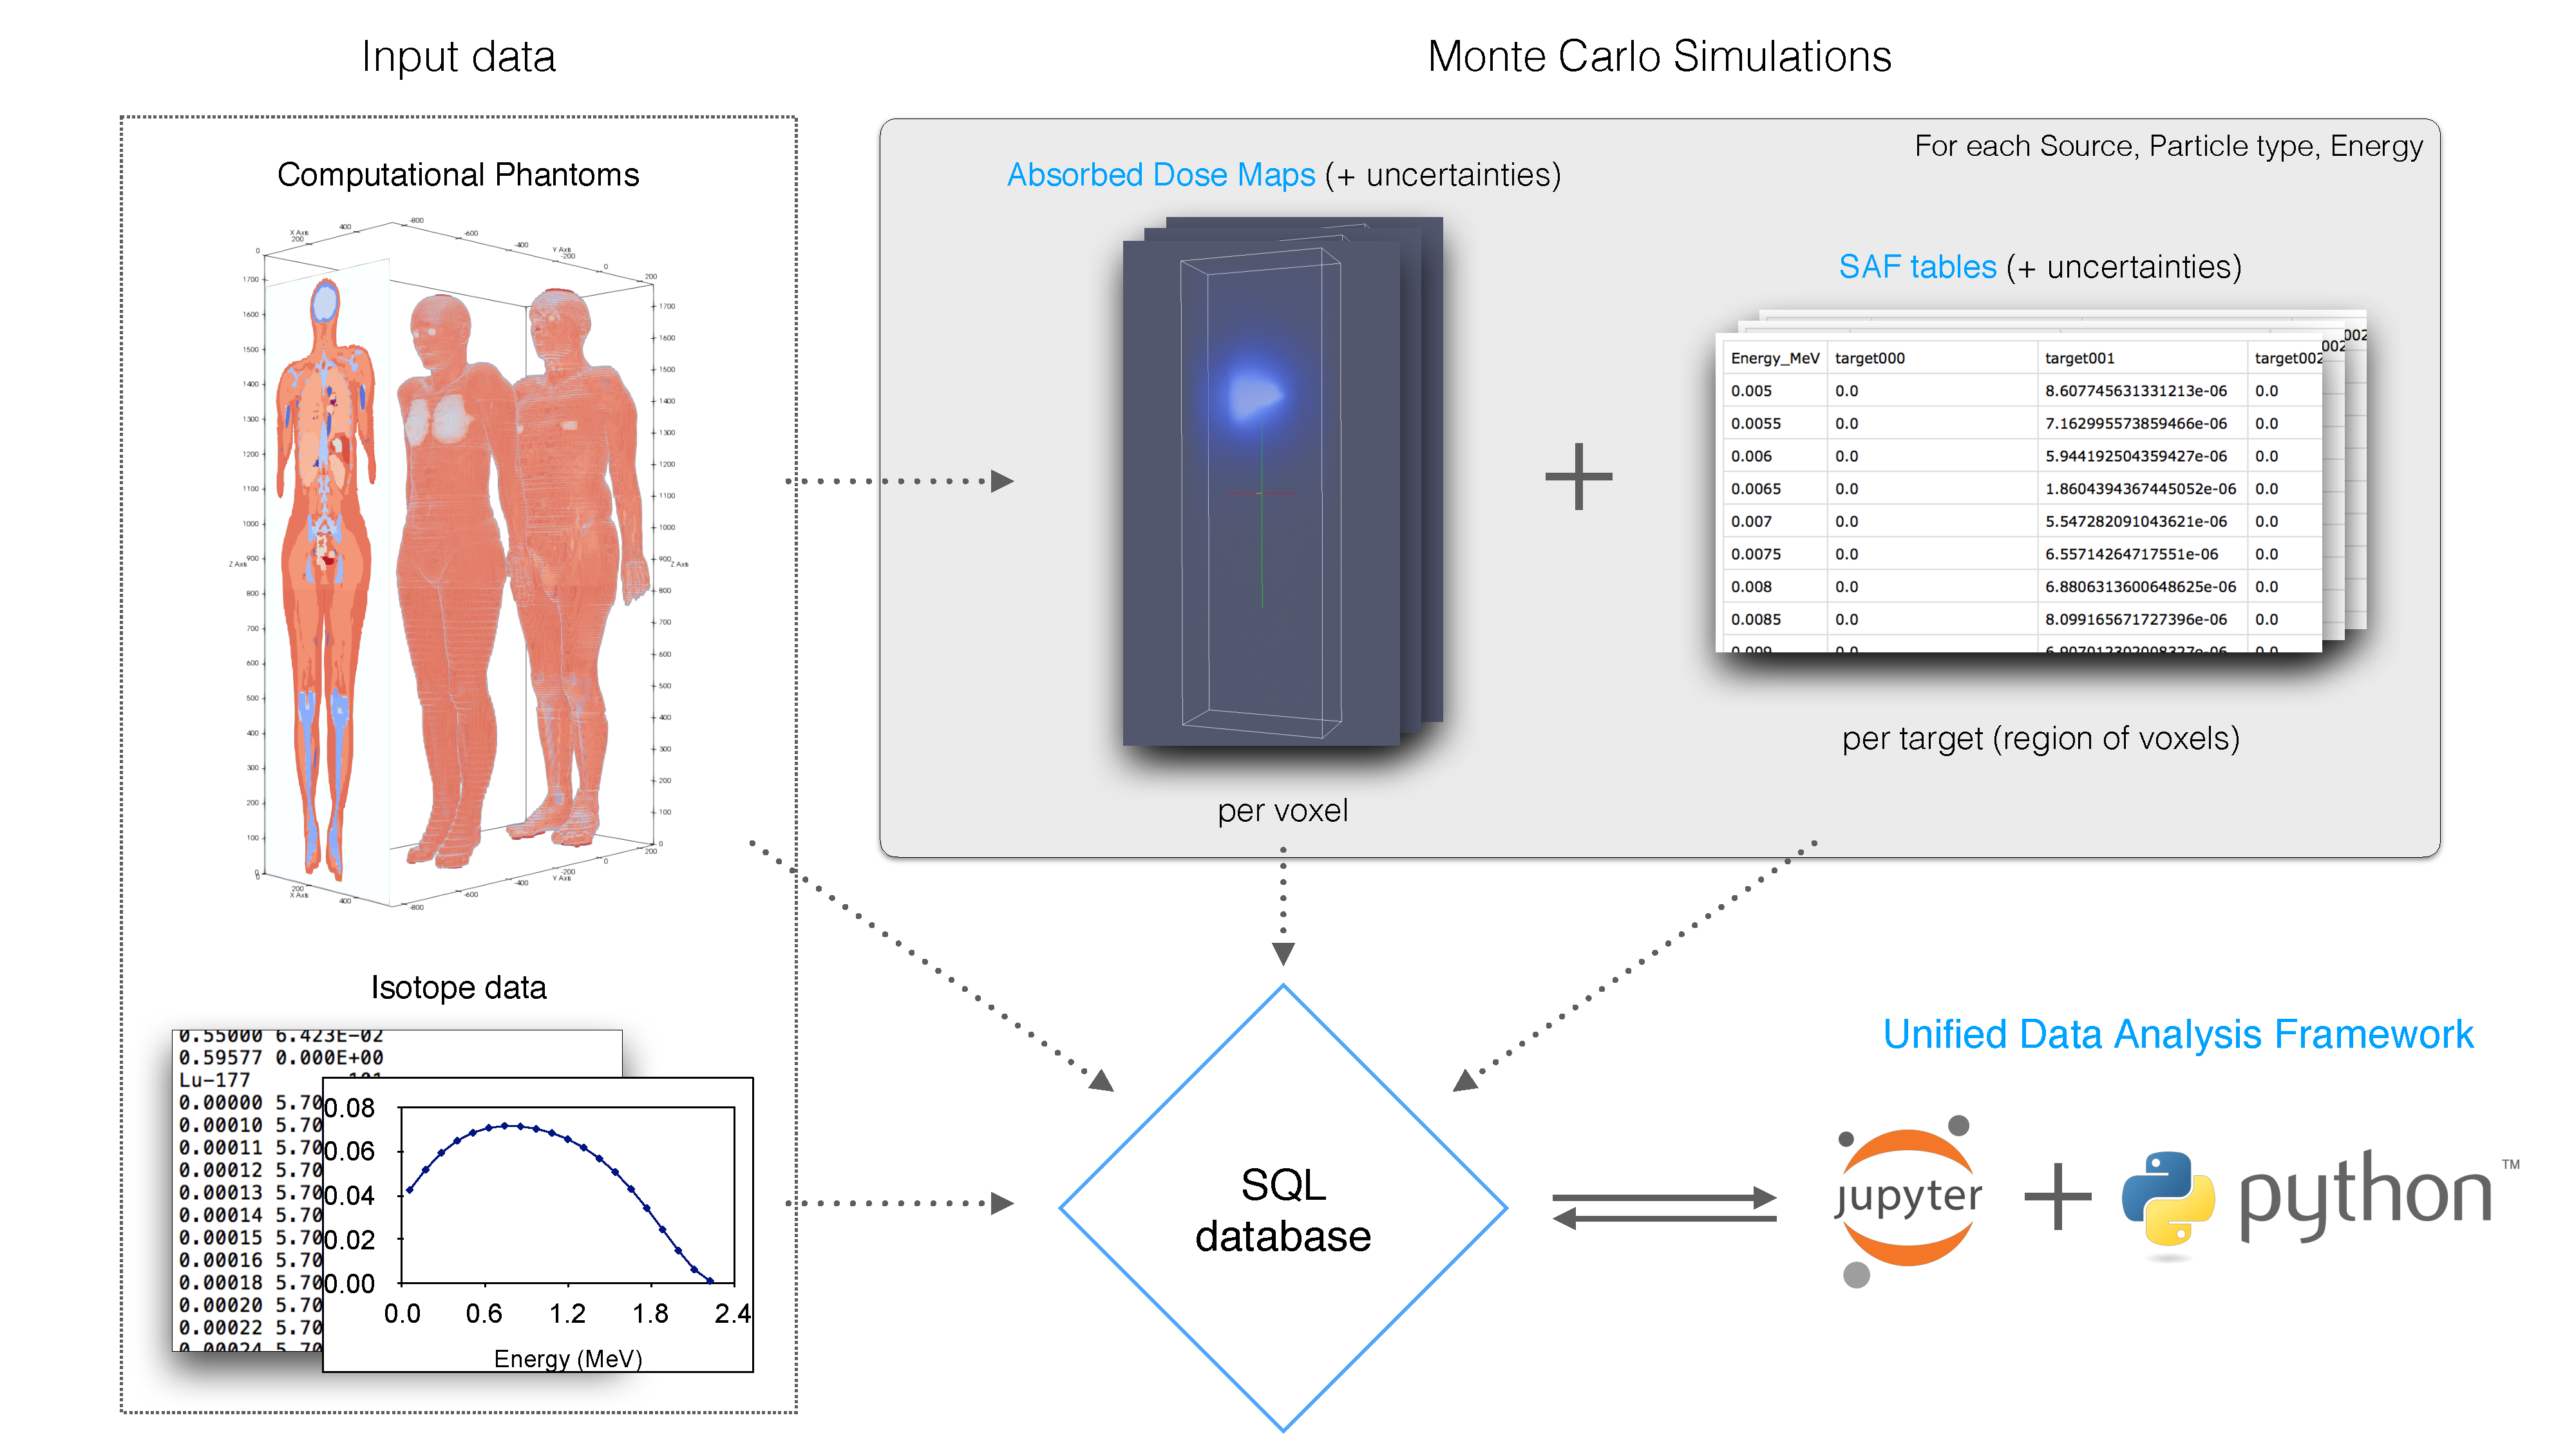
\includegraphics[width=1.0\textwidth]{images/opendose_framework.pdf}
    \caption{OpenDose project overall framework including the unified data
    analysis to be developed in this task.}
    \label{fig:opendose_framework}
  \end{figure}
  
  By building a set of tools to access and process data, this will ensure the
  production of traceable and reproducible dosimetric data for the OpenDose
  project members.

  Another major aspect of the OpenDose collaboration is to provide an open
  access to the generated dosimetric data. For that purpose a website is under
  development to allow data download and simple dosimetry calculations. For
  users who need more advanced calculations, a dedicated Jupyter workspace will
  provide a set of tools to easily access, process and display the OpenDose
  data.

  The task includes the following activities:
  \begin{compactitem}
  \item Developing tools to work seamlessly on the SQL database holding the
    dosimetric data.
  \item Developing data analysis tools using the Python data science ecosystem
    where possible.
  \item Developing visualization tools, exploring Widgets inside the Notebook
    for interactivity.
  \item Evaluate the relevance of Jupyter Notebooks from user feedback
  \item Disseminating results.
  \item Providing support to users.
  \end{compactitem}
  First, these developments will be available to users as Jupyter Notebooks to
  be run locally on their machines. In a second time, these Notebooks will be
  ported on the European Binder instance following developments of task
  \taskref{eosc}{eu-binder}. The reproducibility of generated results will be
  ensured by archiving the software environment with developments of task
  \taskref{ecosystem}{reproducibility}.

  The deliverable of this task will be a demonstrator
  (\localdelivref{opendose-analysis}) available via the EOSC hub, contributing
  to the development of innovatives services for the scientific community.

  The evaluation of the developed tools from user feedback will contribute to
  the deliverable \localdelivref{applications-report}.

  \TODO{How does this task relate to EOSC-life?}

\end{task}

\begin{task}[
  title=Application: Interactive Mathematics with Jupyter Widgets,
  id=math,
  lead=UPSUD,
  PM=17, % UPSUD:16, QS:1, EGI: 1
  wphases={0-36},
  partners={EGI,EP,QS}
  ]

  \TODO{Ideas to reinforce the ties with EOSC services welcome!}

  Computations have played a long time and ever increasing role for
  research and teaching in (pure) mathematics, to explore, search and
  check for conjectures, or better understand algorithmic ideas. This
  led to the development of a whole ecosystem of mathematical
  software, many of which are open source. Given the huge variety of
  mathematical objects and workflows, the Read-Eval-Print-Loop (REPL)
  paradigm -- on which Jupyter is based -- is particularly suitable:
  the user interacts with the system by typing commands that use its
  library of mathematical features, often combined with personal code.
  In fact, the REPL and notebook paradigms of Jupyter as well as some
  of its interactive features were largely inspired by that of
  computer algebra systems such as Maple, Mathematica, or SageMath.

  One major action of the OpenDreamKit project was to foster the
  convergence between the Jupyter and math software ecosystems:
  nowadays Jupyter can be used as a uniform user interface for most
  major systems: e.g. GAP, OSCAR, Pari/GP, SageMath, Singular, and
  even for C++ libraries. This interface is being widely adopted: for
  example, Jupyter has become the standard user interface for
  SageMath, enabling to phase out its former bespoke notebook; by now,
  thousands of jupyter notebooks for SageMath are publicly shared
  (6000+ on GitHub alone).

  Thanks to this prior art, the mathematical community will
  immediately enjoy all the benefits brought by EOSC-based generic
  Jupyter services, including eased collaboration, sharing, archival,
  and reproducibility.

  The next step to maximize attractivity and impact in the
  mathematical community, and this is the aim of this task, is to go
  beyond the REPL paradigm, and \textbf{leverage the real time
    interactivity and flexibility brought by Jupyter widgets for
    Mathematical purposes}. Think making it easy for a teacher or
  researcher to build and disseminate via the EOSC a mini applications
  or dashboard enabling the graphical exploration of a whole range of
  mathematical inputs, with real-time visualization of the associated
  outputs.

  The unique challenge comes from the huge variety of mathematical
  objects that the user may want to visualize and interact with, and
  the variety of graphical representations. Co-design is central here,
  as building a bespoke interactive visualization entails a
  combination of technology skills (e.g. javascript development) and
  business knowledge (designing the interaction and visualization).
  The role of Research Software Engineers is to leverage the
  technology by encapsulating the technical difficulties into flexible
  and easy to use tool boxes from which mathematicians can build
  mini-applications tailored to their needs.

  Within OpenDreamKit, we conducted experiments to explore this
  venue~\cite{ODK_D4.16}. One specific focus was to enable not only
  \emph{interactive visualization}, but also \emph{interactive
    editing}: being able to graphically modify the mathematical object
  being visualized; this enable the interactive exploration of how the
  modifications affect its properties, or to use the editor as input
  widget for a larger applications or dashboards. The outcome of this
  task are the development of two prototypes in SageMath
  (\software{sage-combinat-widget}, a library of widgets for
  combinatorics, and \software{sage-explorer} a generic dashboard for
  interactive browsing and introspection of mathematical objects), and
  contributions to \software{Francy}, an Interactive Discrete Math
  Framework for \software{GAP} and \software{SageMath}.

  The aim of this task is to build on this experience to further
  develop and promote the use of Jupyter widgets for interactive
  Mathematics. This will include the following actions:
  \begin{compactitem}
  \item Engage with the community through tutorials, workshops, online
    discussions, for codesign and for dissemination of the outcomes.
  \item Tackle hurdles to real-time interactivity, typically by
    modernizing the existing 2D and 3D visualization tools in
    SageMath. % E.g.: We don't use Matplotlib's integration in Jupyter
  \item Bring \software{sage-combinat-widgets} and
    \software{sage-explorer} from usable prototypes to standard tools,
    and further contribute to the development of the \software{Francy}
    framework.
  \item Develop other generic mathematical widgets according to the
    users popular requests.
  \item Demonstrate the value all of the above through applications in
    research and teaching.
  \end{compactitem}
  The work carried over will be reported on in~\localdelivref{math}.
\end{task}

% template for a task
% each task should be added to exactly one workpackage
% in the workpackage task list
\begin{task}[
  title=Demonstrator: Reproducible photon science workflows at European XFEL,
  id=reproducibility-xfel,
  lead=XFEL,
  PM=35,
  wphases={7-48},
  partners={EGI,INSERM,SRL,UPSUD}
  ]

  This task (see page \pageref{sec:concept-demonstrator-photonscience}
  for context) includes the following activities:
  \begin{compactitem}
  \item Use the software archive for reproducible computation
    (as co-developed in \taskref{ecosystem}{reproducibility}), with
    the aim to provide reproducible computation environments for data analysis at
    European XFEL that remains executable for the same duration as the
    data is kept (currently aiming at 10+ years, at least 5 years).

    As is common in computational science, software used at XFEL often
    relies on specific combinations of libraries, in many cases with
    particular version requirements. Thus we will need a dedicated
    software archive that holds all relevant packages and source codes
    that are required to build the required computational environments
    (see \taskref{ecosystem}{reproducibility}) to ensure they are
    available even if an open source software provider decides to
    remove their repositories, or changes the API of a package, or
    GitHub decides to terminate their business.

    Applying the work from \taskref{ecosystem}{reproducibility} in the
    context of a production system will demonstrate its true utility,
    and provide important feedback for the design. There will be
    iterative feedback and refinement of the service.

  \item Extend the use of notebooks from \emph{interactive} data
    exploration and analysis at European XFEL to also provide
    computational work flows via (semi-)automatic execution of
    notebooks as described above. The work done in
    \taskref{core}{collaboration} will allow us to execute notebooks in
    the background, and to connect to the running notebook process to
    display or inspect progress, or to modify such a notebook if the
    science requires it.

    By doing so, we can make the standard analysis that is carried out
    by the facility available on EOSC as a service. By using one tool
    (the notebook) we simplify processes for users and for the research
    facility.

  \item Use the work from \taskref{ecosystem}{jupyter-widgets} on
    state-preserving widgets to provide GUI-like elements in notebook
    where interactive user input, data exploration or parameter
    modification is required.

  \item Explore use of the Voila capability to provide
    data exploration dash-boards to lower barriers of working with the
    data (will only be possible for somewhat standard experiments).

  \item Work with the PaNOSC project \cite{panosc} to evaluate and use
    these new and EOSC-enabled services for other Photon and Neutron
    Science research facilities.
  \item Develop a demonstrator (Deliverable \localdelivref{demonstrators}).

  \item Evaluate the chosen workflow design and experience from using
    it in a real-world context; make this available as a report and
    through presentations/workshops to interested organisations and
    facilities. (\localdelivref{applications-report}).




  \end{compactitem}

 \end{task}

\end{tasklist}



\begin{wpdelivs}
%\TODO{update due date and startup!}
%\TODO{update milestone!}

  \begin{wpdeliv}[due=12,miles=startup,id=codesign-support,dissem=PU,nature=R,lead=SRL]
    {Initial requirements for the demonstrators}
  \end{wpdeliv}

  \begin{wpdeliv}[due=24,miles=prototype,id=local-services,dissem=PU,nature=R,lead=EP]
    {Report on the developments of the demonstrator services deployed locally}
  \end{wpdeliv}

  \begin{wpdeliv}[due=36,miles=community,id=demonstrators,dissem=PU,nature=DEM,lead=EGI]
    {Demonstrators based on locally developed services made accessible
      through EOSC. Demonstrators may be developed further subsequently}
  \end{wpdeliv}

  \begin{wpdeliv}[due=48,miles=final,id=applications-report,dissem=PU,nature=R,lead=XFEL]
    {Evaluation of demonstrators and case studies. Report on
      feasibility and user feedback to guide EOSC service design}
  \end{wpdeliv}

\end{wpdelivs}
\end{workpackage}
%%% Local Variables:
%%% mode: latex
%%% TeX-master: "../proposal"
%%% End:

%  LocalWords:  workpackage wphases wpobjectives wpdescription pageref wpdelivs wpdeliv
%  LocalWords:  dissem mailinglists swrepository final-mgt-rep compactitem swsites ipr
%  LocalWords:  TOWRITE tasklist delivref
